Mirko is a big fan of crop circles, geometrical formations of flattened crops that are supposedly of alien origin.

One summer night he decided to make his own formation on his grandmother's meadow. The great patriot that he is, Mirko decided to make a crop formation that would have the shape of the shield part of the Croatian coat of arms, which is a $5 \times 5$ chessboard with $13$ red squares and $12$ white squares.


\includegraphics{aliens1.png}

The chessboard part of the Croatian coat of arms. Grandma's meadow is a square divided into $N \times N$ cells. The cell in the lower left corner of the meadow is
represented by the coordinates $(1, 1)$ and the cell in the upper right corner is represented by $(N, N)$.

Mirko decided to flatten only the grass belonging to red squares in the chessboard, leaving the rest of the grass
intact. He picked an odd integer $M \ge 3$ and flattened the grass so that each square of the chessboard comprises
$M \times M$ cells in the meadow, and the chessboard completely fits inside the meadow.

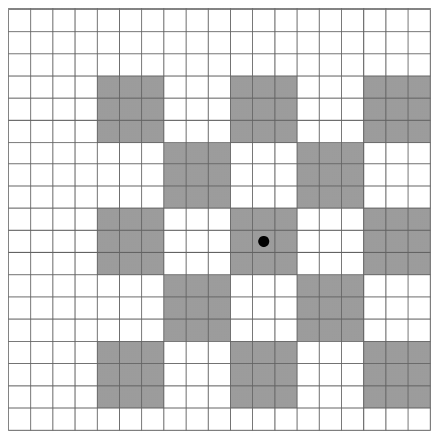
\includegraphics{aliens2.png}

Example meadow and Mirko's crop formation, with $N = 19$ and $M = 3$.
Cells with flattened grass are shown in gray. The center of the formation is at $(12, 9)$ and is marked with a black point.

After Mirko went to sleep, his peculiar creation drew the attention of real aliens! They are floating high above the meadow in their spaceship and examining Mirko's crop formation with a simple device. This device can only determine whether the grass in a particular cell is flattened or not.

The aliens have found one cell with flattened grass and now they want to find the center cell of Mirko's masterpiece, so that they may marvel at its beauty. They do not know the size $M$ of each square in Mirko's formation.

Write a program that, given the size $N$  of the meadow, the coordinates $(X_0, Y_0)$ of one cell with flattened grass, and the ability to interact with the alien device, finds the coordinates of the center cell of
Mirko's crop formation.

The device may be used at most $300$ times in one test run.